\chapter{Systematic Studies of the Numerics of Bath Observables with
  HOPS}
\label{chap:numres}
After developing the tools for obtaining information about bath
related observables in \cref{chap:flow} and the means for their
verification in \cref{chap:analytsol}, we are now in a position to
apply those results.

The roadmap is the following. Using \cref{chap:analytsol} we will
verify the results of \cref{chap:flow} in \cref{sec:hopsvsanalyt}.  A
striking phenomenon will be noticed and explained in a brief detour
\cref{sec:pure_deph}.

In the generic case where no analytic solution we nevertheless are
able to obtain consistent results as is demonstrated in
\cref{sec:prec_sim}.

These results will strengthen the confidence in
the method so that we can turn to more complicated applications.
First a brief overview of interesting features of quantum
thermodynamics is given in \cref{sec:basic_thermo}. Subsequently we
will turn to two applications to demonstrate these features in
\cref{sec:singlemod,sec:otto}.

An overview and explanation of the codes used in this chapter can be found
in \cref{sec:code}.

\section{Some Remarks on the Methods}
\label{sec:meth}
Before we begin with the applications in earnest, let us review some
technical details.

The figures presented may feature error funnels whose origin is,
unless otherwise stated, estimated from the empirical standard
deviation of the calculated quantities due to the finite sample
size. As the quantities that are being calculated using HOPS are
essentially Monte Carlo integrals, those statistical errors scale as
\(1/\sqrt{N}\) with the sample size \(N\) and therefore controllable
besides being simple to estimate. Note however, that a certain number
of samples is required to estimate the standard deviation of a single
trajectory correctly.

To tell whether some vector quantities\footnote{For example a time
  series.} \(X_1, X_2\) obtained with HOPS or otherwise are compatible
with each other or an analytical result, we consider the quantity
\(Δ=X_1 - X_2\). Assuming all numerical errors are negligible, we
demand that \(\abs{Δ} \leq σ_Δ\) for at least \(68\%\) of the entries
of the \(X_i\), where \(σ_Δ\) is the standard deviation due to the
stochastic sampling. This percentage is often displayed in legends as
a number in parentheses.

For the estimation of mean and standard deviation from trajectory
data, Welford's online algorithm is employed to avoid catastrophic
numerical cancellation~\cite{Welford1962Aug,Knuth1997}.

In all simulations discussed an Ohmic spectral density
\begin{equation}
  \label{eq:ohmic_sd}
  J(ω)=η ω \eu^{-\frac{ω}{ω_{c}}}\quad (ω>0)
\end{equation}
is used unless otherwise. This spectral density models an environment
with a physical energy spectrum that is bounded from below and allows
the application of the finite temperature method described
in~\cite{RichardDiss} and \cref{sec:lin_finite}. Also, \(J(0) = 0\)
ensures that there is a unique zero temperature state of the
bath. In~\cite{Kolar2012Aug} it is argued (under weak coupling
assumptions), that \(J(ω)\approx ω^γ\) with \(γ<1\) could lead to a
violation of the third law.  Physically, a scaling of the spectral
density \(\propto ω\) is connected to acoustic
phonons~\cite{Kolar2012Aug}.

In \cref{eq:ohmic_sd} \(η\) is a scaling
constant and \(ω_c\) (the cutoff frequency) regulates the decay of the
spectral density. The corresponding bath correlation function (BCF)
is
\begin{equation}
  \label{eq:ohmic_bcf}
  α(τ) = \frac{1}{π} ∫\dd{ω} J(ω) \eu^{-\iu ωτ} =
  \frac{η}{π}\qty(\frac{ω_c}{1+\iu ω_c τ})^2.
\end{equation}
We see that higher cutoff frequencies correspond to a faster decay of
the bath correlation function. This parameter provides control over
the ``Markovianity'' of the bath.

It may be remarked, that~\cref{eq:ohmic_bcf} does not correspond to a
simple sum of exponentials. As such it exercises the HOPS method and
serves as a model for a general bath correlation function. For use
with HOPS, a sum of exponentials must be fitted to the BCF. In
\cref{sec:hopsvsanalyt} we will see, that this is indeed a valid
strategy.

Throughout this chapter, we will only apply the nonlinear
method~\cite{Hartmann2017Dec} described in \cref{sec:nmqsd_basics}
(see also \cref{sec:nonlin_flow}).

\section{Comparison with an Analytical Solution}
\label{sec:hopsvsanalyt}
In \cref{chap:analytsol} and specifically \cref{sec:oneosc,sec:twoosc}
an analytical solution for a quantum Brownian motion like model was
derived. Using this solution, we are able to verify the results of
\cref{chap:flow} and benchmark the HOPS method. It will be shown, that
HOPS can indeed reproduce the \emph{exact} open system dynamics of the
bath energy flow.

\subsection{A Harmonic Oscillator coupled to a single Bath}
\label{sec:oneosccomp}
We begin with the simplest possible model of a single zero temperature
bath.  For the simulations with HOPS the model
\cref{eq:one_ho_hamiltonian} was made dimensionless by choosing
\(Ω=1\). Simulations were run for both for zero temperature and a
finite temperature with varying bath correlation functions.

\begin{figure}[t]
  \centering
  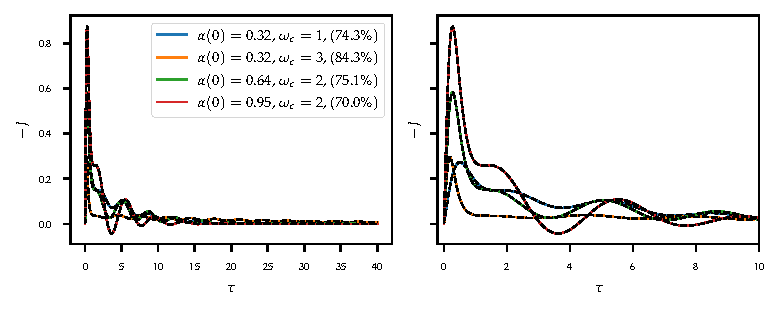
\includegraphics{figs/analytic_comp/flow_comp_zero.pdf}
  \caption{\label{fig:comp_zero_t} The bath energy flow \(-J\) for
    different parameters of the ohmic bath correlation function
    \cref{eq:ohmic_bcf}. The solid lines have been obtained with HOPS
    and the dashed lines using the analytic solution. A good agreement
    is evident visually and corroborated by the consistency values in
    the legend (see \cref{sec:meth} for an explanation).  The
    simulation with \(ω_{c}=3\) (orange) stands out for its slow long
    term decay, whereas the same simulation with longer bath
    correlation time (blue) initially decays much slower but falls
    below its orange counterpart for longer times.}
\end{figure}
\paragraph{Zero Temperature}
The bath energy flow \(J=-∂_t\ev{H_\bath}\), from here on called
simply ``the flow'' or ``bath energy flow'', for the zero temperature
case are illustrated in \cref{fig:comp_zero_t}. The results agree to a
very good accuracy, validating the findings of \cref{chap:flow}.

Although the simulations are primarily intended as a benchmark for
HOPS and a verification for the results of \cref{chap:flow} some
observations can be made in \cref{fig:comp_zero_t}.

First, the flows for different parameters all feature the
characteristic spike originating from the ``initial slip'', as
explained in \cref{sec:pure_deph}. This is a quite universal feature
and also shows up on a single trajectory level suggesting that it is
not strictly related to an energy exchange with the bath but rather to
the build-up of interaction energy. This will be discussed further in
\cref{sec:one_bath_cutoff}.

Note that the model \cref{sec:oneosc} used here is missing a so-called
counter term, that is often prescribed to obtain a stokes like,
velocity dependent friction term in the equations of motion and takes
the form \cite{Weiss2008Mar}
\begin{equation}
  \label{eq:counter_term}
  H_{\mathrm{C}} \sim ∑_{λ}\frac{\abs{g_{λ}}^{2}}{ω_{λ}} q^{2}.
\end{equation}
When \cref{eq:counter_term} is included in \cref{sec:oneosc} it
becomes the Caldiera-Legget Model.

This counter term balances the renormalization of the system potential due
to the bath. It is therefore an interesting question how the initial
slip behaves in its presence.

The time dependence of the flow also varies both with the shape of the
BCF and the coupling strength. For longer correlation times
\(τ_{B}\propto 1/ω_c\) we find that the flow initially decays much
slower at the same coupling strength (blue and orange lines) and
exhibits stronger oscillations. After this initial period the
situation is reversed. For large coupling strengths we can observe a
``backflow'' of energy out of the bath. In all cases the flow features
some oscillations and decays to zero which is physical for the
situation of a harmonic oscillator that loses most of its energy into
a zero temperature bath.

The observed behaviour for longer bath memories may be qualitatively
understood by assuming that the system interacts with the same part of
the bath for a longer time and can therefore more efficiently transfer
energy. When the bath memory is short however, new interactions have
to be built up continuously which leads to a slower energy
transfer. Correspondingly, the system energy decays slower for shorter
bath memories \cref{fig:ho_zero_entropy}. Another explanation is a
resonance effect due to the peak of the BCF being located at \(ω_c\)
and the HO energy gap being one. We will discuss this point further in
\cref{sec:one_bath_cutoff} in the context of another model.

\begin{figure}[htp]
  \centering
  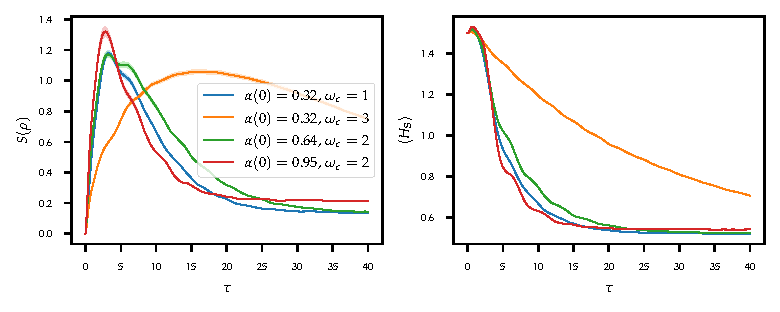
\includegraphics{figs/analytic_comp/entropy_zero.pdf}
  \caption{\label{fig:ho_zero_entropy} Left panel: The von Neumann
    entropy of the system state as a measure for entanglement with the
    bath. Right panel: The system energy as a function of time. The
    \(ω_{c}=3\) case (orange) is markedly different from the others,
    with a much slower decay of the system energy and slower entropy
    dynamics. The strongest coupling simulation (red) converges to a
    markedly different steady state.}
\end{figure}
The ``backflow'' observed in \cref{fig:comp_zero_t} for stronger
coupling seems to diminish the advantage of stronger coupling over
larger bath memories. The decay of the red curve in the right panel of
\cref{fig:ho_zero_entropy} is barely faster than the decay of the blue
curve, despite much larger coupling strength in the case of the red
curve. This may be due to the system interaction ``too long'' with a
given portion of the bath. Here we observe this behaviour for stronger
coupling which shortens the time-scale of energy exchange. In
\cref{sec:one_bath_cutoff} we will see, that these oscillations occur
generically for long bath memories and stronger coupling, and that
energy transfer performance is strongly dependent on timing.

Note however, that the steady state is not a product state as can be
seen by the residual entropy in \cref{fig:ho_zero_entropy} in the
cases where the steady state has been approximately reached. The
stronger the coupling, the larger the entanglement. The \(α(0)=0.95\)
simulation appears to be leading to a qualitatively different steady
state than the one with the same cutoff but weaker coupling
strength. This also manifests in a higher expected system energy in
the steady state.

The time dependence of the entropy the expectation value of the system
energy is markedly different for \(ω_c=3\). Although the coupling
strength is larger than in the \(α(0)=0.32,\, ω_c=1\) case the energy
loss of the system is much slower and the initial energy gain is
less pronounced. This is consistent with the flow in
\cref{fig:comp_zero_t}.

The simulation was run with a hierarchy depth of \(\norm{\vb{k}} \leq 5\)
(simplex truncation\footnote{see \cref{sec:hops_basics}}) and a BCF
fit with \(7\) terms taken from \cite{RichardDiss} which was also used
in the analytical solution. The harmonic oscillator Hilbert space was
truncated to \(15\) dimensions. As the initial state the first excited
state of the oscillator was chosen. Some \(N=5000\) trajectories have
been computed and lead to a quite satisfactory statistical error that
is small enough to be invisible in \cref{fig:comp_zero_t}. The
normalized standard deviation of the bath energy flow follows the
usual one-over-square-root rule as is illustrated in
\cref{fig:sqrt_conv}. Even after just \(N=1000\) trajectories the
relative statistical error is on the order of \(10^{-3}\).
\begin{figure}[htp]
  \centering
  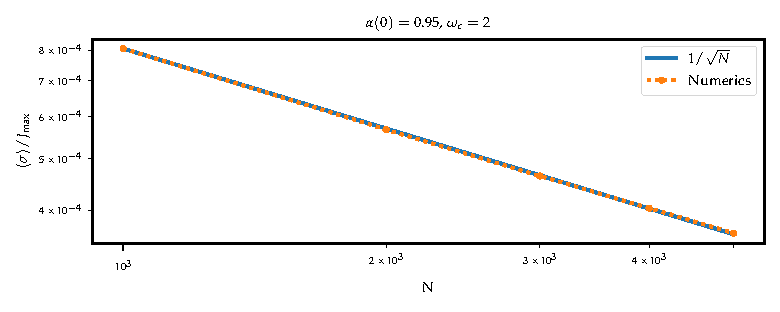
\includegraphics{figs/analytic_comp/sqrt_convergence.pdf}
  \caption{\label{fig:sqrt_conv} The (empirical) standard deviation
    (the statistical error) of the flow for the last configuration in
    \cref{fig:comp_zero_t} normalized by the maximum absolute value of
    \(J\). The \(1/\sqrt{N}\) rule is obeyed to good accuracy showing
    that the estimation of the variance is sound.}
\end{figure}
\begin{figure}[htp]
  \centering
  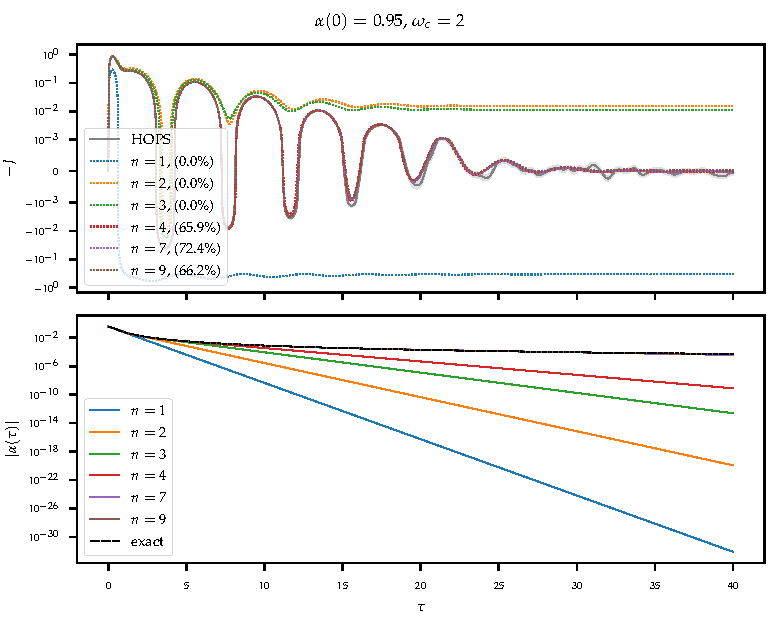
\includegraphics{figs/analytic_comp/analytical_terms_important.pdf}
  \caption{\label{fig:analytical_terms_important} Upper Panel: The
    analytical solution for the zero temperature bath energy flow
    using different numbers of terms in the BCF expansion in a
    symmetric logarithmic scale. For \(7\) terms the consistency
    (number in parentheses) with the numerical solution is best. For
    \(n<4\) the results are unphysical in the steady state.  Lower
    Panel: The absolute value of the approximated bath correlation
    function.}
\end{figure}

The analytical solution is quite sensitive to the quality of the BCF
expansion.  While one might expect that choosing the same number of
terms in the expansion for the analytical solution as was used for the
HOPS simulation, there still remains a systematic difference between
HOPS and the analytical solution, as the stochastic processes is
sampled using the full bath correlation function and applying more
intricate numerical approximations~\cite{RichardDiss}.  Nevertheless,
the best agreement is found for using the same number expansion terms
in both HOPS and the analytical solution as is illustrated in
\cref{fig:analytical_terms_important}. Note that the consistency value
given in \cref{fig:analytical_terms_important} is slightly different
from the one in \cref{fig:comp_zero_t}, as here a separate fit was
made rather than using the fit from \cite{RichardDiss}.

Interestingly, the solutions using a BCF expansion with three terms or
fewer lead to an unphysical non-zero steady state bath energy
flow. Considering specifically the case of one expansion term this may
be related to the fact that now the BCF term so that
\(α(τ)=G \exp(-Wτ)\) is related to a Lorentzian spectral density that
also includes unphysical negative frequencies. To correctly reproduce
the steady state, the fit must model the decay of the BCF correctly on
the appropriate time scales.
\fixme{additional curve in plot, idea: start in the zero state ->
  product state is not the steady state, maybe longer times}

\paragraph{Finite Temperature}
\begin{figure}[t]
  \centering
  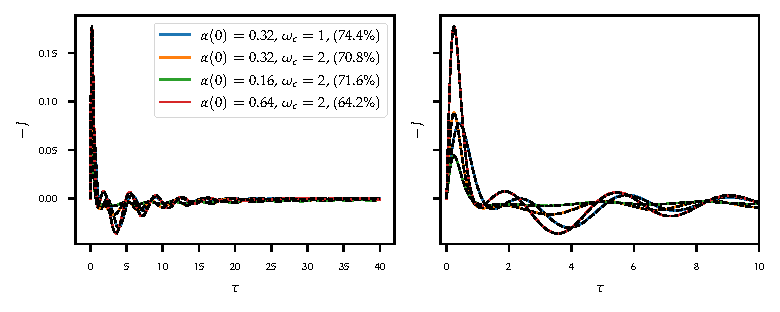
\includegraphics{figs/analytic_comp/flow_comp_nonzero.pdf}
  \caption{\label{fig:comp_finite_t} The bath energy flow \(-J\) of
    the quantum Brownian motion model for different parameters of the
    ohmic bath correlation function \cref{eq:ohmic_bcf} in the finite
    temperature \(T=1\) case. The presentation is equivalent to
    \cref{fig:comp_zero_t}.}
\end{figure}
The results for the finite temperature case are illustrated in
\cref{fig:comp_finite_t} for a temperature of \(T=1\). The setup was
otherwise equivalent to the zero temperature simulations, except for
the number of trajectories which was chosen to be \(N=10^5\).  Again
the high consistency values suggest that the findings of
\cref{chap:flow} are valid. The last case (\(α(0)=0.64,\, ω_c=2\)),
falls just short of the \(68\%\) mark, but agrees very well
visually. It is very probable, that simply more samples are
required.\fixme{maybe re-run...}

We find a similar behaviour to the zero temperature case, but this
time with a more pronounced flow out of the bath as it has a nonzero
energy expectation value. For higher coupling strengths, the flow
amplitude is higher, as is also the case for lower cutoffs.

One potentially contestable point in \cref{chap:flow} was the
appearance of the time derivative of the thermal stochastic process in
\cref{eq:pureagain}. The numerical method which is used to sample the
stochastic processes allows for a straight forward implementation of
this derivative so that no numerical derivatives are required and
there appears to be no problem.

As the dimensionality of the Monte Carlo integral underlying the
NMQSD/HOPS formalism is increased by the ``Stochastic Hamiltonian''
method, we observe markedly slower convergence as the variance of the
individual trajectories is higher. In \cref{fig:cons_dev_finite} the
convergence behaviour, as well the consistency with increasing
trajectory count are plotted and this behaviour is observed. We also
find that in the more challenging regimes of stronger coupling or
longer bath correlation times the behaviour of the convergence is more
volatile, dipping into regions of inconsistency even at high sample
counts. While the mean difference between the numerical and the
analytical flow is always below the mean statistical error, larger
fluctuations can occur at certain points in time when a new region of
the probability space is sampled.

\begin{figure}[p]
  \centering
  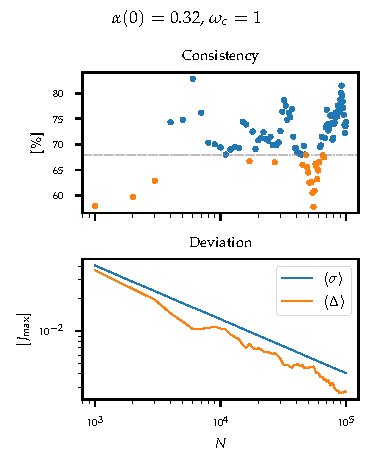
\includegraphics{figs/analytic_comp/consistency_development_0.pdf}
  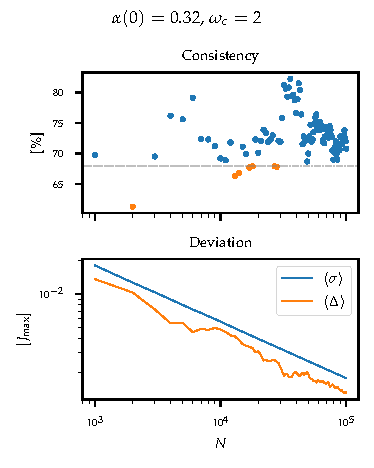
\includegraphics{figs/analytic_comp/consistency_development_1.pdf}
  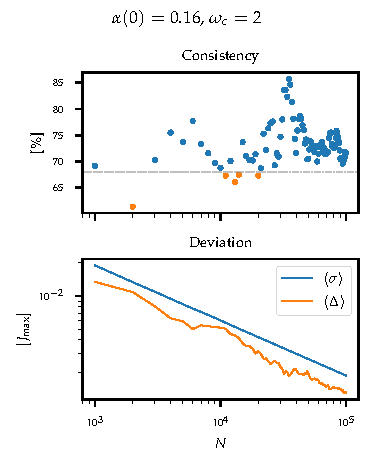
\includegraphics{figs/analytic_comp/consistency_development_2.pdf}
  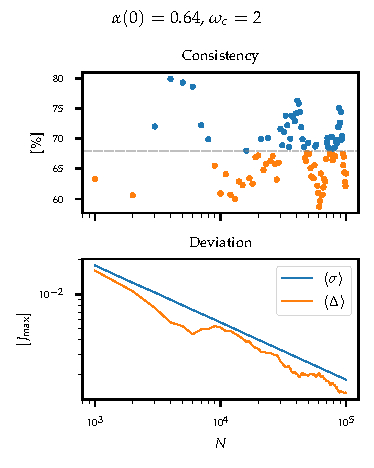
\includegraphics{figs/analytic_comp/consistency_development_3.pdf}
  \caption{\label{fig:cons_dev_finite} The convergence of the flows of
    \cref{fig:comp_finite_t} with increasing trajectory count. The
    upper panels show the consistency, where the grey line marks the
    \(68\%\) threshold for consistency. The lower panel shows the time
    averaged values of the statistical error \(\ev{σ}\) and the
    deviation from the analytical result \(\ev{Δ}\) by the maximum
    absolute value of \(J\). In the last plot, the consistency
    development is quite unstable despite the mean deviation from the
    analytical result being smaller than the mean standard
    deviation. In all cases these two curves scale with the
    \(1/\sqrt{N}\) rule.}
\end{figure}

% The advantage of the ``Stochastic Hamiltonian'' method for finite
% temperature (see \cref{eq:thermalh}) is that one doesn't have to deal
% with the finite temperature BCF that does decay markedly slower than
% its zero temperature counterpart as is illustrated in
% \cref{fig:bcf_decay}. Generically, more terms in the BCF expansion
% would be required to capture the algebraic decay appropriately.

% \begin{figure}[t]
%   \centering
%   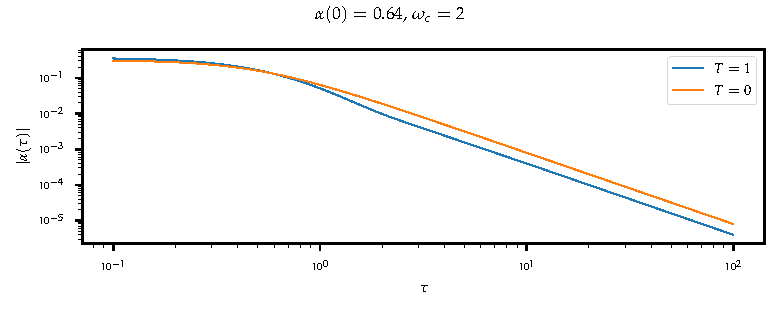
\includegraphics{figs/analytic_comp/bcf_decay.pdf}
%   \caption{\label{fig:bcf_decay} The absolute value of the Ohmic BCF
%     used in the last simulation of \cref{fig:comp_zero_t}.}
% \end{figure}

\subsection{Two coupled Harmonic Oscillators coupled to two Baths}
\label{sec:twoosccomp}
We now progress to a slightly more complicated setting, namely that of
two oscillators coupled to two baths\footnote{This also constitutes
  the first application of the TU-Dresden TQO group's HOPS code-base
  to multiple baths.}. As noted before, multiple baths are an
important ingredient for interesting models like quantum-thermodynamic
engines. At the same time, this setting is much more numerically
challenging as the number in BCF expansion terms doubles, which in
turn increases the number of hierarchy states.

The model of \cref{sec:oneosc} was generalized to two oscillators
coupled to two separate baths in \cref{sec:twoosc} and
\cref{eq:hamiltonian_two_bath}. In this section we simulate this model
and compare the results with the analytical solution.

For simplicity, the parameters were chosen symmetric so that the
frequencies of both oscillators are the same \(Ω=Λ=1\). As before,
\(Ω\) defines the energy unit. The zero temperature bath correlation
functions of both baths were chosen identically with a cutoff
frequency \(ω_c=2\). The intra-oscillator coupling was chosen as
\(γ=0.5\). The hierarchy was truncated so that \(\abs{\vb{k}}\leq 3\) and a BCF
expansion with five terms was chosen to limit memory demands and
\(10^{4}\) trajectories were integrated.

To limit the variance the temperature of one of the baths was set to
zero, so that only one thermal stochastic process was introduced. The
other bath was chosen to have \(T=0.6\). The ground state of the
system Hamiltonian \(\ket{0}\otimes \ket{0}\) was chosen as the
initial state of the oscillators.

The main challenge of simulating the model \cref{eq:hamiltonian_two_bath} is
the dimension of the system Hilbert space which is constrained by the
available memory. In the simulation discussed here, each oscillator
was truncated at \(9\) levels leading to \(9^2 = 81\) dimensions in
total\footnote{This is a naive method of truncation, but sufficient
  for the purposes of this work.}. The effect of a too drastic
truncation of the system Hilbert space can be seen in
\cref{fig:insufficient_levels}. At the temperature chosen the mean
level occupation of a harmonic oscillator is given by the Bose distribution
\begin{equation}
  \label{eq:harm_mean_occ}
  \ev{n} = \frac{1}{\eu^{Ωβ}-1} \approx 0.23 < 1.
\end{equation}
Nevertheless, quite more than two levels are required per
oscillator. This may be due to a required minimal resolution of the
position operators that occur in the model
\cref{eq:hamiltonian_two_bath} which is formulated with position space
in mind.

The final result can be studied in \cref{fig:sufficient_levels}. We
find good, but not excellent agreement. Based on the results of
\cref{sec:oneosccomp} however, it can be argued that this result is
sufficient to corroborate the validity of the results of
\cref{sec:multibath}. With more computational effort\footnote{Mainly
  more BCF expansion terms.} and fine-tuning of parameters an even
better agreement between the analytical and the numerical results may
be achieved.
\begin{figure}[htp]
  \centering
  \begin{subfigure}[t]{.49\linewidth}
    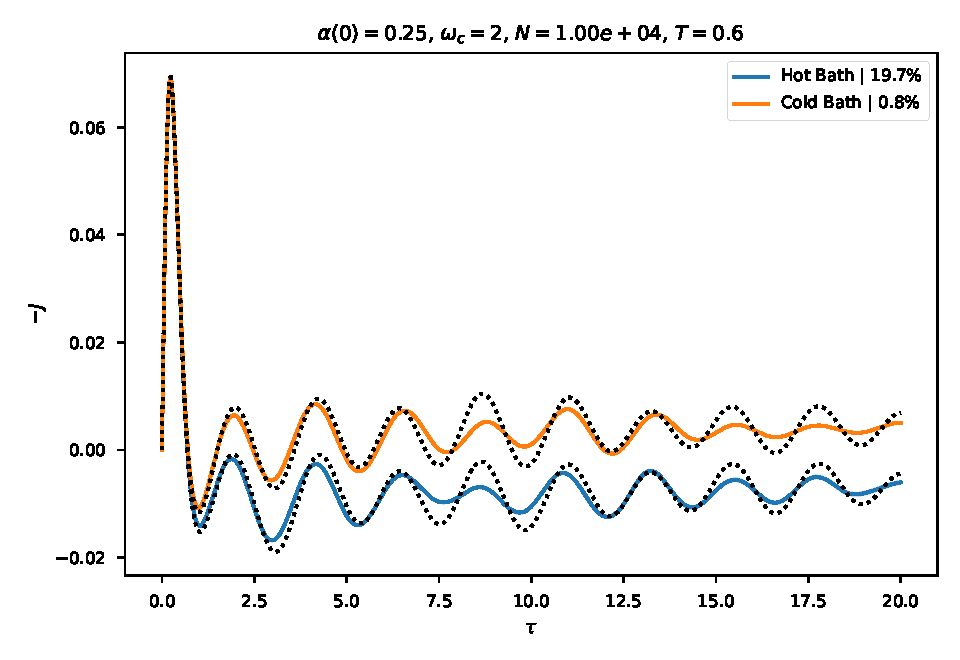
\includegraphics{figs/analytic_comp/comparison_two_5bcf_5ho.pdf}
    \caption{\label{fig:insufficient_levels}\(\dim\hilb_\sys=25\).}
  \end{subfigure}
  \begin{subfigure}[t]{.49\linewidth}
    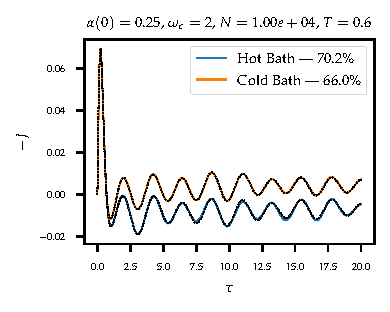
\includegraphics{figs/analytic_comp/comparison_two_ho.pdf}
    \caption{\label{fig:sufficient_levels}\(\dim\hilb_\sys=81\).}
  \end{subfigure}
  \caption{\label{fig:comp_two_bath} The bath energy flows for
    the model \cref{eq:hamiltonian_two_bath}, where the dashed lines
    correspond to the analytical solutions.}
\end{figure}

\Cref{fig:comp_two_bath} exhibits some interesting features. The
initial slip peak in the bath energy flows is identical for both baths
and independent of temperature as suggested by the discussion in
\cref{sec:pure_deph}. As is expected, the hot bath looses energy and
the cold bath gains energy, while this process is modulated by the
intra-oscillator coupling. It follows from the analytical solution
that eventually a steady state without oscillations will be reached.

The zero temperature bath flow converges very much faster than the
finite temperature flow despite the whole system being connected, at
least indirectly, to the hot bath. The reason for this is that the
derivative of the thermal stochastic process \(\dot{ξ}\) dominates the
variance of the flow for each trajectory. This is also the reason that
expressions depending on the hierarchy states rather than time
derivatives of stochastic processes are preferred as discussed in
\cref{sec:general_obs}.

We have shown that the findings of \cref{chap:flow} are consistent
with \cref{chap:analytsol} and that through a careful choice of the
HOPS parameters such as hierarchy depth, Hilbert space dimension and
BCF expansion the exact open system dynamics of the bath energy flow
can be reproduced. The statistical error can be made arbitrarily small
by increasing the trajectory count. For a given target error, the
trajectory count can be estimated by the empirical standard deviation
of a given observable.

For future work there remains the generalization of the work in this
section and \cref{chap:analytsol} to time dependent couplings and
Hamiltonians. Because the NMQSD and also HOPS are largely agnostic of
these factors, we may safely assume that the results of the comparison
will be similar to the ones presented here.

\section{Pure Dephasing and the Initial Slip}
\label{sec:pure_deph}
As seen in \cref{fig:comp_finite_t,fig:comp_zero_t,fig:comp_two_bath},
the short time behavior of the bath energy flow is dominated by
characteristic peak at short times. Because this peak occurs at very
short time scales, it may in part be explained by a simple calculation
which neglects the system dynamics by setting \(H_\sys=0\).

We solve the model with the Hamiltonian (Schr\"odinger picture)
\begin{equation}
  \label{eq:puredeph}
  H = L^†(t) B + L(t) B^† + H_\bath
\end{equation}
with \(L(t)=L(t)^†\), \([L(t), L(s)] = 0\;\forall t,s\) (so that
Heisenberg Hamiltonian matches \cref{eq:puredeph}) and \(B,\,H_\bath\)
as in \cref{sec:nmqsd_basics}.

Because \([L,H]=0\) we can immediately solve \(L_H(t)=L_S(t)\), where
the subscript distinguishes the Heisenberg and Schr\"odinger pictures
respectively. The Heisenberg equations for the \(a_λ\) yield
\begin{equation}
  \label{eq:alapuredeph}
  a_λ(t) = a_λ(0) \eu^{-\iu ω_λ  t} - \iu g_λ^\ast∫_0^t\dd{s} L(s)
  \eu^{-\iu ω_λ  (t-s)}.
\end{equation}

This allows us to calculate
\begin{equation}
  \label{eq:pureflow}
  \dot{H}_\bath =\iu\comm{H_{\inter}}{H_{\bath}} = - ∑_λ g_λ L(t) \qty[∂_t a_λ(0) \eu^{-\iu ω_λ t} - \iu
  g_λ^\ast∫_0^t\dd{s} L(s) ∂_t \eu^{-\iu ω_λ (t-s)}] + \hc,
\end{equation}
which gives with a state of the form \(ρ=\ketbra{ψ} \otimes ρ_β\)
(\(ρ_β\) being a thermal state)
\begin{equation}
  \label{eq:pureflowexpectation}
  \ev{\dot{H}_\bath } = -2 ∫_0^t\dd{s}\ev{L(t)L(s)} \Im[\dot{α}(t-s)].
\end{equation}
For time independent \(L\) this becomes
\begin{equation}
  \label{eq:pureflowtimeindep}
  \ev{\dot{H}_\bath } = -2 \ev{L^2} \Im[α(t)].
\end{equation}

The proportionality to the imaginary BCF \(α\) does explain the
initial peak in the bath energy flow. The imaginary part of the BCF is
zero for \(t=0\) and then usually features a peak at rather short
times (assuming finite correlation times). For the ohmic BCF used here
and shown in \cref{fig:ohm_bcf_ex}, this feature is very prominent.
\begin{figure}[htp]
  \centering
  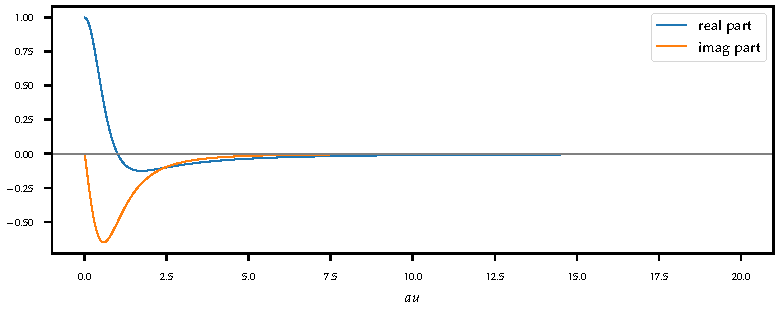
\includegraphics{figs/misc/ohmic_bcf_example.pdf}
  \caption{\label{fig:ohm_bcf_ex} An ohmic BCF with \(ω_{c}=η=1\). The
  imaginary part has a peak at the beginning and decays to zero.}
\end{figure}

Generically, the imaginary part of the BCF is negative at least for
short times as it takes the form
\begin{equation}
  \label{eq:negtive_imag}
  \Im[α(τ)] = -\frac{1}{π}∫_{0}^{τ}J(ω) \sin(ωτ)\dd{ω}
\end{equation}
which is negative for \(τ\leq π/ω_{\mathrm{max}}\), where
\(ω_{\mathrm{max}}\) is a characteristic cutoff frequency of the
system. The direction of the initial slip flow for unmodulated systems
will therefore be always be into the bath compensating for negative
interaction energy.

Interestingly, \cref{eq:pureflowexpectation} does not contain any
reference to the temperature of the bath. Therefore, the bath energy
can only surpass its initial value in this model, as the dynamics
match the zero temperature case in which the bath has minimal energy
in the initial state.

A thermodynamically useful model should feature significant system
dynamics that do not commute with the interaction or modulation so
that the Hamiltonian does not commute with itself at different
times. Coupling that is not self-adjoint \fixme{plot: if time, i could
  do the energy shovel with non-hermitian} may also have this effect,
but in the literature most effective qubit models tend to favour
Hermitian couplings
\cite{Aurell2019Apr,Hita-Perez2021Nov,Hita-Perez2021Aug,MacQuarrie2020Sep,Andersen2017Feb,Mezzacapo2014Jul}. For
the spin-boson system, non Hermitian coupling it is the result of the
random phase approximation, which however does not imply weak
coupling~\cite{Irish2007Oct}.

For completeness, the interaction energy is given by
\begin{equation}
  \label{eq:pureinter}
  H_\inter = L(t)\qty[∑_λg_λ\qty(a_λ(0)\eu^{-\i ω_λ t} - \i
  g^\ast_λ∫_0^t\dd{s} L(s) \eu^{-\i ω_λ (t-s)})] + \hc,
\end{equation}
yielding
\begin{equation}
  \label{eq:pureinterexp}
  \ev{H_\inter} = 2 ∫_0^t\dd{s}\ev{L(t)L(s)} \Im[α(t-s)].
\end{equation}

For time independent coupling we have
\begin{equation}
  \label{eq:pureinterexp_timeidp}
  \ev{H_\inter} = 2 \ev{L^2} \int_{0}^{t}\Im[{α}(s)]\dd{s} = -Δ\ev{H_{\bath}}.
\end{equation}

It may be useful to normalize the BCF based on \cref{eq:pureinterexp},
so that the pure interaction energy build-up in the initial slip is
taken as measure of interaction strength. To make the normalization
independent of \(L(t)\), we choose the normalization to be
\begin{equation}
  \label{eq:bcfnorm}
  \begin{aligned}
  \mathcal{N} &= 2 \abs{\frac{\max_t\norm{L(t)L^\dag(t)+\hc}}{\max_t{\norm{H(t)}}} ∫_0^∞ \Im[α_u(τ)]\dd{τ}}\\
    α(τ) &= α_u(τ)/\mathcal{N},
  \end{aligned}
\end{equation}
where \(α_u\) is some unnormalized BCF. This normalization has the
useful property, that it neutralizes any scaling in \(L\). Note that
here the convention in which \(α\) is dimensionless is used.

% this is not true
% imaginary part becomes proportional to the Dirac delta in the limit
% where typical cutoff frequency \(ω_c\rightarrow ∞\). The integral over
% the real part of \(α\) always gives zero if the spectral density obeys
% \(J(0) = 0\) and tends to exhibit fast oscillations and fast decay in
% the large-cutoff limit. For weak coupling, it may therefore be
% neglected. This constitutes the Markov limit mentioned in
% \cite{Strunz2001Habil}.
The Ohmic-type BCF is
\begin{equation}
  \label{eq:normohmic}
  α(τ)=\frac{ω_c  s }{ (\max_t\norm{H})(1+\iu ω_c τ)^{s+1}},
\end{equation}
in this normalization.

\section{Precision Simulations of the Zero Temperature Spin-Boson Model}
\label{sec:prec_sim}
Despite being solvable analytically, the models from
\cref{sec:hopsvsanalyt} are numerically cumbersome, as their system
Hilbert space is infinite dimensional and has to be truncated. In this
section we concern ourselves with a very simple model that poses
lesser numerical challenges and still exhibits interesting behaviour.

Both the performance of the HOPS method itself
(\cref{sec:stocproc,sec:trunc}) and the characteristics of the flow
mediated by the concrete form of the bath correlation function
(\cref{sec:one_bath_cutoff,sec:one_bathcoup_strength}) will be
investigated. We will find that the numerics do indeed yield very
consistent results and that the specifics of the energy flow depend
very much on the spectral density.

As an analytical solution to a given open system is generally not
known, another indicator of the proper choice of HOPS parameters is
required. Upon the example of a single qubit coupled to a single zero
temperature bath, we will study the convergence behaviour of the
interaction energy.  The corresponding Hamiltonian is
\begin{equation}
  \label{eq:one_qubit_model}
  H = \frac{1}{2} σ_z + \frac{1}{2} ∑_λ\qty(g_λ σ_x^† a_λ + g_λ^\ast
  σ_x a_λ^†) + ∑_λ ω_λ a_λ^\dag a_λ,
\end{equation}
where we have chosen \(H\) to be dimensionless\footnote{The energy scale
is set by the system Hamiltonian.}.

In the language of HOPS this corresponds to \(H_\sys=σ_z/2\),
\(L=σ_x/2\). We again choose the Ohmic BCF as explained in
\cref{sec:meth}. Throughout this section we choose the ``up'' state
\(H_S\ket{1} = 1/2\ket{1}\) as the initial state of the system.

The main measure of convergence for variables other than the
trajectory count are consistency conditions. One check available to us
is energy conservation which allows us to calculate the expectation
value of the interaction energy through integration of the bath energy
flow. The interaction energy obtained in this way can then be compared
to the interaction energy obtained directly as shown in
\cref{sec:intener}. Note that this scheme may also be adapted easily
to multiple baths where the sum of interaction energies has to be
considered and to time dependent Hamiltonians where finite power has
to be taken into account.

The main sources of systematic deviations for the model
\cref{eq:one_qubit_model} are the quality of the sampling of the
stochastic process and the cutoff of the hierarchy. The first becomes
important when the cutoff frequency is large and the BCF vanishes
rapidly and has to be resolved on shorter time scales. The second is
important when the cutoff frequency is smaller and the bath has a
longer memory.

\subsection{Stochastic Process}
\label{sec:stocproc}
For studying the convergence behaviour regarding the sampling of the
stochastic process we chose the cutoff as \(\norm{\vb{k}} \leq 4\)
(simplex truncation\footnote{see \cref{sec:hops_basics}}),
\(N=4.5 \cdot 10^5\) trajectories and an Ohmic BCF with \(α(0)=1.6\)
and \(ω_c=4\).  The sampling method uses the ``Fast Fourier
Transform'' (FFT) as described in~\cite{RichardDiss}. As the system
Hilbert space dimension is small, a BCF expansion with seven terms was
employed.

The main parameter of this method is the accuracy of the FFT. The
implementation compares the BCF and its FFT approximation on the time
interval of the simulation and chooses the internal
parameters\footnote{The number of time grid points and the integral
  boundaries in frequency space.} so that the difference normalized by
\(α(0)\) is smaller than a given value \(ς\).

\begin{figure}[htp]
  \centering
  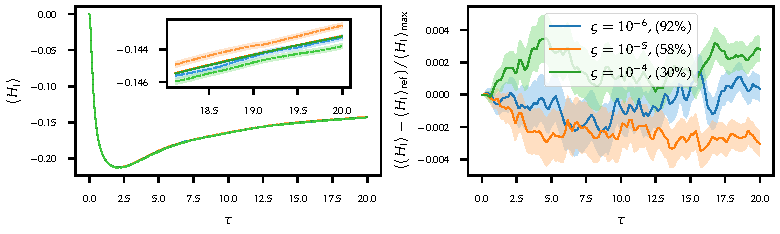
\includegraphics{figs/one_bath_syst/stocproc_systematics_interaction}
  \caption{\label{fig:stocproc_systematics} Left panel: The
    interaction energy of the model \cref{eq:one_qubit_model} for
    \(α(0)=1.6\) and \(ω_c=4\) using different precisions for the
    sampling of the stochastic process. The dashed lines are obtained
    using energy conservation while the solid lines are obtained
    directly as in \cref{sec:intener}. The consistency between the two
    is given in the legend of the right panel. An inset shows the
    curves for the final three time units. Right panel: The difference
    of the interaction energies obtained using energy conservation and
    directly. The values are normalized by the maximal absolute value
    of the interaction energy. The \(\varsigma = 10^{-6}\) case gives
    the most accurate results in terms of energy conservation, but
    when using the direct method of calculating \(\ev{H_{\inter}}\)
    all parameter choices yield the same results.}
\end{figure}
\Cref{fig:stocproc_systematics} illustrates the effect of this
parameter. We find very good qualitative agreement for all values of
\(ς\). The indirectly calculated value of then interaction energy
shows some fluctuation between the settings, but the value calculated
directly is very stable as can bee seen in the inset of
\Cref{fig:stocproc_systematics}.

Only in the \(\varsigma=10^{-6}\) case however, compatibility is
satisfied at the given sample count. This is due to the fact that here
multiple values that are obtained in different ways, namely system
energy and the flow, have to be considered. The system energy depends
on the zeroth hierarchy order only whereas the flow additionally
depends on the first hierarchy states and has to be numerically
integrated.
\begin{figure}[htp]
  \centering
  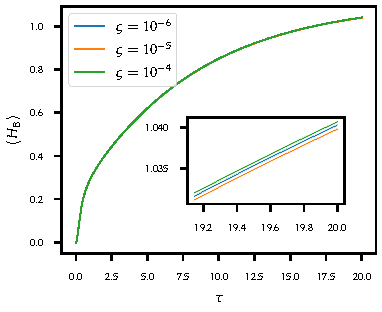
\includegraphics{figs/one_bath_syst/stocproc_systematics_bath_energy}
  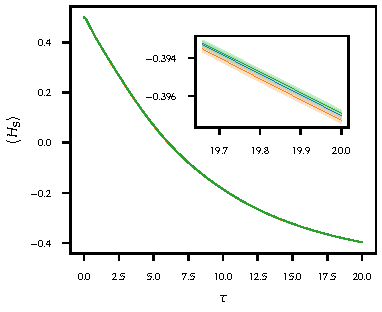
\includegraphics{figs/one_bath_syst/stocproc_systematics_system}
  \caption{\label{fig:stocproc_bath_sys}The bath and system energies of the
    model \cref{eq:one_qubit_model} for \(α(0)=1.6\) and \(ω_c=4\)
    using different precisions \(\varsigma\) for the sampling of the
    stochastic process. Systematic deviations outside the error bounds
  occur mainly in the bath energy.}
\end{figure}

The individual contributions to the indirectly obtained interaction
energy may be studied in \cref{fig:stocproc_bath_sys}. The bath
energy, being an integrated quantity for which errors may accumulate,
is most susceptible to systematic deviations outside the error bounds,
as is clearly visible in the insets. Nevertheless, the qualitative
agreement of the different simulations is excellent.

The development of the consistency of trajectory count \(N\) can be
studied in \cref{fig:stocproc_consistency_dev}. Only for the highest
precision case we have a consistent picture. For lower precision, the
consistency fluctuates and only occasionally surpasses \(68\%\). For
the lower precisions we find that they initially demonstrate
compatibility (until about \(N=10^4\)) but eventually diverge from the
exact\footnote{The result that demonstrates compatibility
  consistently.} result. It is therefore important to consider the
dependence of the compatibility on the sample count \(N\) to judge the
veracity of the simulation results.
\begin{figure}[htp]
  \centering
  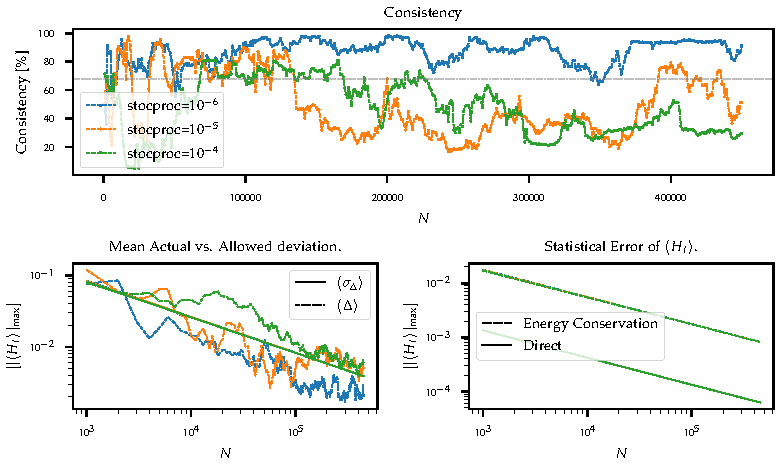
\includegraphics{figs/one_bath_syst/stocproc_systematics_consistency}
  \caption{\label{fig:stocproc_consistency_dev} Upper panel: The
    compatibility (number of values within one standard deviation, see
    \cref{sec:meth}) of the flow (direct computation vs. energy
    conservation) of the model \cref{eq:one_qubit_model} for
    \(α(0)=1.6\) and \(ω_c=4\) using different precisions
    \(\varsigma\) for the sampling of the stochastic process in
    relation to the trajectory count \(N\). Only the
    \(\varsigma=10^{-6}\) simulation is consistent for all sample
    counts. Lower left: The time averaged difference of the direct and
    indirect interaction energies (dashed) and the time averaged
    standard deviation of the difference (solid) as a function of
    trajectory count. Only for the smallest \(\varsigma\) the
    difference is consistently smaller than the standard deviation of
    the difference. Lower right: The time averaged statistical errors
    of the interaction energy calculated directly (solid lines) and
    indirectly through energy conservation (dashed lines). The
    deviation of the direct method smaller by an order of magnitude.}
\end{figure}

Apart from being closer to the correct result, the direct computation
of the interaction energy has the advantage of providing faster
convergence\footnote{See \cref{fig:stocproc_consistency_dev}, lower right
  panel.}.

\subsection{Hierarchy Truncation}
\label{sec:trunc}
As the effect truncation depth has already been studied thoroughly
in~\cite{RichardDiss}, we will keep the discussion short.  We chose
\(N=4.5 \cdot 10^5\) trajectories and an Ohmic BCF with \(α(0)=0.8\)
and \(ω_c=2\). Again, seven a BCF expansion with seven terms have been
used. The coupling strength has been chosen with the help of
\cref{sec:pure_deph}, so that the interaction energy is of a similar
order of magnitude as in the discussion
above. \Cref{fig:k_systematics} suggests that there seems to be no
improvement in accuracy or even change in the value of the flow for
\(\norm{\vb{k}}\geq 4\). However, the inset in the left panel
demonstrates that the direct result differs slightly for
\(\norm{\vb{k}} = 2\), which demonstrates that an adequate choice of
truncation depth is important.
\begin{figure}[htp]
  \centering
  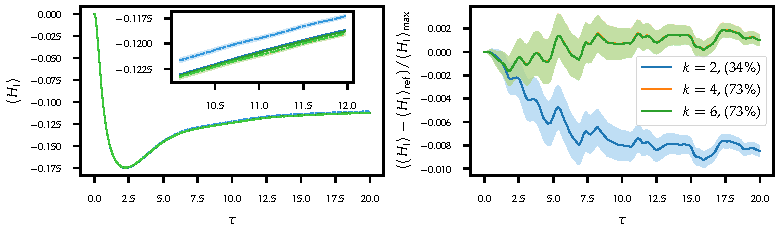
\includegraphics{figs/one_bath_syst/k_systematics_interaction}
  \caption{\label{fig:k_systematics} The same as
    \cref{fig:stocproc_systematics} but for \(α(0)=0.8\) and
    \(ω_c=2\) and for various truncation depths \(k=\norm{\vb{k}}_{\mathrm{max}}\).}
\end{figure}


We see in \cref{fig:k_systematics_system} that the difference of the
\(\norm{\vb{k}} = 2\) case from the \(\norm{\vb{k}} = 6\) is on the
same order of magnitude for system energy and interaction energy. The
bath energy, being an integrated quantity, accumulates errors and
deviates the most. Also, the results for \(\norm{\vb{k}} = 4,6\) agree
perfectly in all cases.
\begin{figure}[htp]
  \centering
  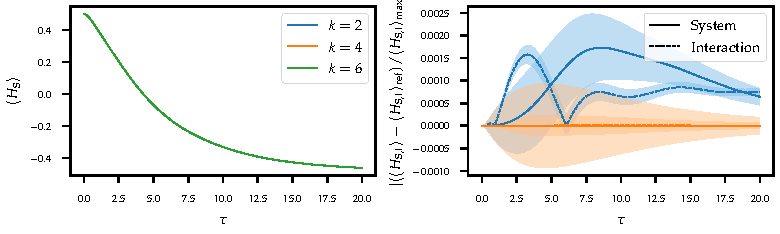
\includegraphics{figs/one_bath_syst/k_systematics_system}
  \caption{\label{fig:k_systematics_system} Left panel: The norm of
    the difference of a single trajectory to the \(\norm{\vb{k}} = 6\)
    case. The solid lines show the difference of the zeroth hierarchy
    states and the dashed lines show the same for the first hierarchy
    states.  There is still a slight difference on the trajectory
    level. Right panel: The difference between the \(k=6\) result and
    the results with \(k<6\) normalized by the maximal absolute system
    energy (solid lines) and the same for the interaction energy
    (dashed lines) as well as the bath energy change (dotted). The
    deviation is most substantial for the bath energy change, as
    errors can accumulate in the integration of the bath energy flow.}
\end{figure}
The left panel of \cref{fig:k_systematics_system} demonstrates, that there is still a
difference greater than the machine epsilon on the level the
trajectories. This difference however, is small enough not to impact
observables much.  The deviation of the system, interaction and bath
energies from the highest precision case (\(k=6\)) is also
plotted.


Summarizing, we conclude that the HOPS parameters have to be chosen
carefully for precision simulations, but that a more relaxed choice of
parameters already give a \emph{very} good qualitative picture.

\fixme{maybe run a simulation with more hierarchy depth and more bcf
  terms, check whether there is a mistake} It remains for future work
to perform a detailed study of the systematics of the finite
temperature flow and modulated Hamiltonians. In the following sections
we will look at some examples of physically interesting systems with
less focus on the systematics of convergence.

\subsection{Varying the Cutoff Frequency}
\label{sec:one_bath_cutoff}
The lessons learned in \cref{sec:stocproc,sec:trunc} will now be
applied to simulate \cref{eq:one_qubit_model} with high consistency
for various parameter choices of the cutoff \(ω_{c}\) of the BCF
\begin{equation}
  \label{eq:ohmic_bcf_repeat}
  α(τ) =
  \frac{η}{π}\qty(\frac{ω_c}{1+\iu ω_c τ})^2.
\end{equation}
Guided by these demonstrations, we'll turn to a more detailed analysis
of the role of non-Markovianity in the energy transfer characteristics
of our model. The quantification of the initial slip dynamics in
\cref{sec:pure_deph} will also be verified.

To make the interaction energies comparable to each other, the BCF
normalization of section \cref{sec:pure_deph} is being used. Because
of the small size of the Hilbert space, we were able to choose a HOPS
configuration\footnote{\(\norm{\vb{k}}\leq 7\), seven BCF terms,
  \(\varsigma = 10^{-6}\)} that yields high-accuracy
results\footnote{A detailed account of the consistency is given in
  \cref{fig:omega_interaction_consistency}.}, based on the results of
the previous section. The only problematic result is the one for
\(ω_c=1\), but there is good qualitative consistency in this case.

For all simulations \(N=5\cdot 10^{5}\) trajectories were integrated
to produce the results that are summarized in
\cref{fig:omega_systematics_system}.
\begin{figure}[htp]
  \centering
  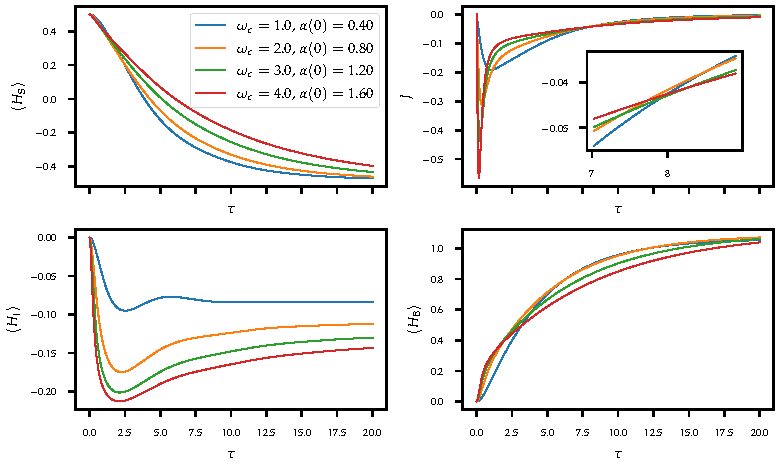
\includegraphics{figs/one_bath_syst/omega_energy_overview}
  \caption{\label{fig:omega_systematics_system} Energy overview for the
    model \cref{eq:one_qubit_model} for various coupling strengths and
     cutoff frequencies. The curves are converged out, and the error
    funnels are not visible.}
\end{figure}

Let us preface the following discussion with a note of caution. All
the discussed phenomena are specific to the minimal model
\cref{eq:one_qubit_model}, although sometimes similarities to
phenomena observed in \cref{sec:hopsvsanalyt} can be seen. Whether
there is some universality to the results obtained is an interesting
question for a more detailed future detailed study.\fixme{Remove this?}

The interaction energy expectation values, despite being in the same
order of magnitude and not in the weak coupling regime, differ
significantly. This illustrates the limitation of the estimate in
\cref{sec:pure_deph} and exemplifies the nontriviality of the open
system dynamics. Better estimates of the interaction energy and thus
interaction strength may be derived from ideas similar to the ones
discussed in \cref{sec:normest}.  Besides the magnitude, the
qualitative time dependence of the interaction energies varies,
especially between the \(ω_c=1\) configuration and the others.

The blue (\(ω_c=1\)) curve exhibits two pronounced turning points in
contrast to the other simulations. This behaviour is a symptom of
interference of the system and bath time scales which are of similar
orders in this simulation, an idea that we will develop further
below. Further, despite having the weakest overall coupling strength
\(α(0)=0.4\) the system energy falls off the fastest after a short
period where it is above the other configurations. This behaviour is
also visible in the bath energy expectation value, where this
simulation almost reaches the same levels as the \(ω_c=2\)
configuration for \(τ\gtrsim 5\).

The flow is generally negative (the bath gains energy) and decays
after an initial peak. All the flow graphs appear to be crossing in
about the same point \(τ\approx 7.7\) after which their ordering by
magnitude is reversed.  The inset shows that the crossing is not
precisely at the same point, nevertheless further investigation of
this phenomenon may of interest in the future. The decay is faster for
higher cutoff frequencies and stronger couplings. Despite the higher
interaction energies and coupling strengths, the high-cuttoff
simulations exhibit a slower energy transfer after the initial peak
has decayed sufficiently, with the system energy falling slower and
the bath energy rising slower. The situation is generally reversed for
short times \(τ\lesssim 2.5\), because here the build-up of
interaction energy is significant.

The presentation in \cref{fig:omega_systematics_system} is not
conducive to comparing the actual performance of the energy transfer,
due to the variable shape of the spectral density and the chosen
coupling strengths. Because the maximum of the Ohmic spectral density
is located at \(ω_c\) the special observed energy transfer behaviour
for \(ω_c=1\) is likely due to a resonance effect (see above) as the
system energy level spacing is unity.

The dissipator of the master equation for this two level system only
depends on the value of the spectral density at the level
spacing~\cite[p. 66]{Rivas2012}\footnote{There \(L=σ_{+}\), but this
  has no bearing on the connection to \(ω_{0}\).}  (\(ω_{0}=1\) here),
so that it is reasonable to expect, that there may be variations
whenever its magnitude at this point changes.  On the other hand, a
strong dependence of the flow on the shape of the bath correlation
function beyond lamb-shift like influences, as we will find below is
an indicator of the departure from the weak coupling limit.
\fixme{Here, some master equation comparison would be nice.}.

\paragraph{Energy Transfer Characteristics}
After focusing on the systematics and achieving very high consistency
in our simulations, we continue to shed some light on the role of bath
memory and resonance in the behavior of the energy transfer between
system and bath.

\begin{wrapfigure}[13]{O}{0.3\textwidth}
  \centering
  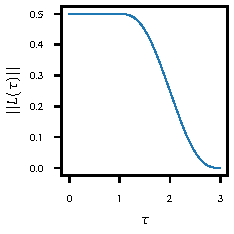
\includegraphics{figs/one_bath_syst/L_mod}
  \caption{\label{fig:L_mod} The smooth modulation of the coupling
    operator \(L(τ)\).}
\end{wrapfigure}
For a systematic study of resonance, we first compare the flow for
shifted ohmic spectral densities\footnote{See \cref{sec:shift_sp} for
  details.} with identical scaling \(α(0)\) and cutoff frequency
\(ω_c=2\). We turn off the interaction smoothly\footnote{A smoothstep
  function of order two with a transition period of two. See
  \cref{sec:smoothstep}.} over two time units before the system has
reached its steady state and compare how much energy has been
transferred in terms of the final bath and system energies and the
loss due to the modulated coupling.

The less energy the system has at the end of the process and the
faster the process concludes, the better the performance of
transfer. If the interaction energies are on the same scale, the
decoupling costs should be roughly the same in terms of total energy
change. Otherwise, they may lead to an additional change of system and
bath energies between the different simulations. Ideally the bath
energy changes to take up any energy added introduced by the
decoupling.

To make space for the shifted bath correlation functions, the system
energy gap has been set to four so that \(α(0)=8\) represents a quite
reasonable coupling strength for our purposes here.

The results for three shifts are presented in
\cref{fig:resonance_analysis}. For all shifts the spectral density has
a finite value at the value of system level spacing, but only in the
\(ω_s=2\) case, the resonance condition is fulfilled. Indeed, the
energy transfer out of the system is the best for the resonant case
(see \cref{fig:resonance_analysis}, middle panel).

The change in total energy due to the decoupling of the bath is
moderately higher than in the resonant case than in the \(ω_s=1\)
case, but the final system energy is the lowest. \fixme{The decoupling
  seems to affect mainly the bath energy (see left panel). Should I
  say so?}
\begin{figure}[htp]
  \centering
  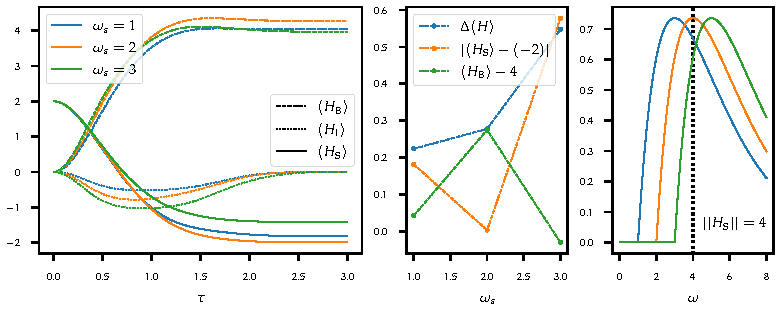
\includegraphics{figs/one_bath_syst/resonance_analysis}
  \caption{\label{fig:resonance_analysis} Left
    panel: The system, bath and interaction energies for various Ohmic
    BFCs with \(α(0)=8,\,ω_c=2\) shifted by \(ω_s\). Mid panel: The
    difference in total energy, the distance of the system energy to
    the ground state energy and the distance of the bath energy to the
    initial system energy. Right panel: The spectral density for the
    three shift values. \(\norm{H_\sys}\) does mean in this case, that
    the energy level spacing of the system is \(4\). There resonant
    case has the best energy transfer behaviour as gauged by the final
    system energy.}
\end{figure}

The third simulation with \(ω_s=3\) exhibits the worst performance
with the highest residual system energy and the highest change in
total energy due the large magnitude of the interaction energy.
Deactivating the interaction lowers the final bath energy in all
cases, but here this effect is most pronounced.

Were the interaction switched off abruptly, the system and bath
energies would remain untouched. Turning the interaction off in finite
time reduces the energy introduced into the system in the cases
discussed here. System and bath energy must therefore compensate part
of the negative interaction energy after the system is decoupled from
the bath. Hence, the observed lowering of system and bath energy after
decoupling. However the effect can also act into the other direction
as we shall see below.

The \(ω_{s}=1\) case exhibits the smallest cost in terms of total
energy change.  The small change in the total energy is due to the
magnitude of the interaction energy, which is the smallest compared to
the other to shifts.

Interestingly, if we modulate the system periodically with angular
frequency \(Δ\), also bath frequencies of \(ω_{0} + n Δ\)
(\(n\in\NN\)) become important, so that shifting the spectral density
to higher frequencies is advantageous, as we will find out in
\cref{sec:modcoup_reso}.

% Turning of the interaction leads mostly to a reduction of the final
% bath energy (see the middle panel).  This effect will also appear in
% most of the cases discussed below. When deriving a master equation for
% this two level system~\cite[p. 68]{Rivas2012}, there occurs a lamb
% shift term that acts as a correction to the unitary evolution of the
% system. Turning the interaction off adiabatically removes this leads
% to a change in what one may define as system energy in this case. In
% the case discussed here, the coupling is not weak so that this
% explanation may only serve as a means of analogy. Compensating for the
% negative interaction energy, the system and bath energy expectation
% value both fall when the coupling is turned off.\fixme{is this
%   reasonable?}

% For an ohmic spectral density the lamb shift energy is
% \begin{equation}
%   \label{eq:lshift_twolevel}
%   2Δ=\eu^{-1/ω_{c}}\,\mathrm{Ei}\qty(\frac{1}{ω_{c}}) - ω_{c},
% \end{equation}
% which is negative for all the cases discussed here and may account for
% some part of the negative interaction energy. In this way, the removal
% of the bath would

\begin{wrapfigure}[16]{O}{0.4\textwidth}
  \centering
  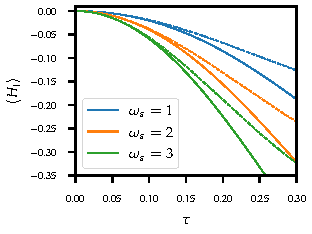
\includegraphics{figs/one_bath_syst/initial_slip_resonance}
  \caption{\label{fig:initial_slip_resonance} The interaction energies
    (solid lines) of the models in \cref{fig:resonance_analysis} and
    the predictions for the interaction energy due to the initial slip
    dynamics \cref{eq:pureinterexp_timeidp} (dashed lines). Larger
    frequency shifts of the spectral density lead to a higher
    magnitude of the interaction energy and faster dynamics.}
\end{wrapfigure}
Generally the maximal absolute interaction energy is roughly
proportional to the shift, so that the short term interaction strength
as measured by the interaction energy expectation value is not only
dependent on the width and total norm of the spectral density, but
also on its absolute distribution in frequency space. The shift adds a
phase factor \(\eu^{-\i ω_{s} τ}\) to the BCF which makes the
imaginary part steeper. This in turn leads to faster initial slip
dynamics and a speed buildup of interaction energy as demonstrated in
\cref{fig:initial_slip_resonance}. The observed effect is sensible on
an intuitive level as higher frequency oscillators are being excited
in the bath leading to faster dynamics.

Due to the asymmetry of the spectral density, the simulations for
\(ω_s=1\) and \(ω_s=3\) are not directly comparable. A repetition of
this investigation with a (pseudo~\cite{Mukherjee2020Jan}) Lorentzian
spectral density and for different interaction
time-frames\footnote{steady state vs. transient states} is left for
future work.

The longer term picture is being studied in
\cref{fig:resonance_analysis_steady}. We see broadly similar energy
transfer characteristics for \(ω_{s}=1\) and \(ω_{s}=2\), where the
off-resonant case may be slightly advantageous. The left panel shows,
that although the system energy before the decoupling is lower in the
resonant case, the situation is reversed during the decoupling as now
also the system energy is affected by the process and the interaction
energy of the off-resonant case is slightly larger in
magnitude. However these effects are quite marginal and should be
taken with care. The system energy difference amounts to
\(\Delta\langle H_\mathrm{S}\rangle=0.00397\pm 0.00010\), but only the
statistical error has been taken into account. The simulations were
run with \(N=10^{4}\) trajectories and the same HOPS settings as in
the discussion above, so that some confidence may be placed in them.

For \(ω_{s}=3\) the approximate steady state has not been reached yet
and the energy transfer is incomplete and the residual system energy
is the highest. The fast growth of the interaction energy leads to a
slower initial loss of system energy. On longer time scales we see a
slow, almost linear transfer of energy from the system into the
interaction. The system dynamics are catching up with the bath.
\begin{figure}[htp]
  \centering
  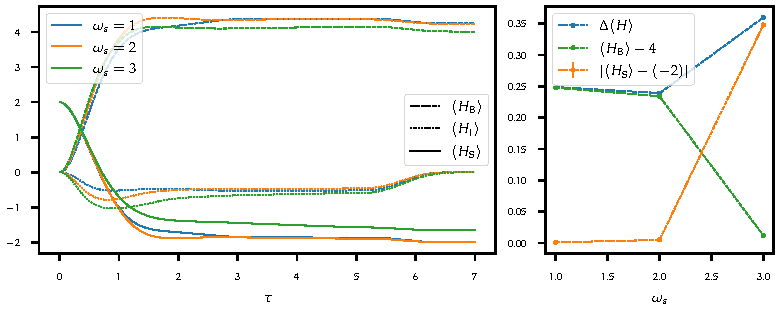
\includegraphics{figs/one_bath_syst/resonance_analysis_steady}
  \caption{\label{fig:resonance_analysis_steady} The same as
    \cref{fig:resonance_analysis} but for a longer coupling time.}
\end{figure}

To study the effect of the bath memory, we use Ohmic spectral
densities with linearly spaced \(τ_{\bath}\equiv ω_c^{-1}\) that have
been shifted and scaled by numerical optimization so that their peaks
coincide and the resulting maximal absolute interaction energies
identical. The rightmost panel of \Cref{fig:markov_analysis} shows
plots of the spectral densities obtained. We can see, that not only
the magnitude at resonance point enters, as the peak heights are quite
different. We will encounter this behavior again in
\cref{sec:extr_mem}.

The results that can be obtained are very much dependent on the
timing. \Cref{fig:markov_analysis} has been arrived at by tweaking the
time point of decoupling so that an extremum in the system energy of
the long memory (\(τ_{B}=1\)) case is captured. This leads to an
advantageous transfer performance with a lower system energy and
similar cost in terms of total energy change, although residual system
energy is still higher than in \cref{fig:resonance_analysis_steady}.
Although initially the system energy falls fastest for the short
memory case the situation is reversed after about \(τ=0.5\).
\cref{fig:resonance_analysis_steady}.
\begin{figure}[htp]
  \centering
  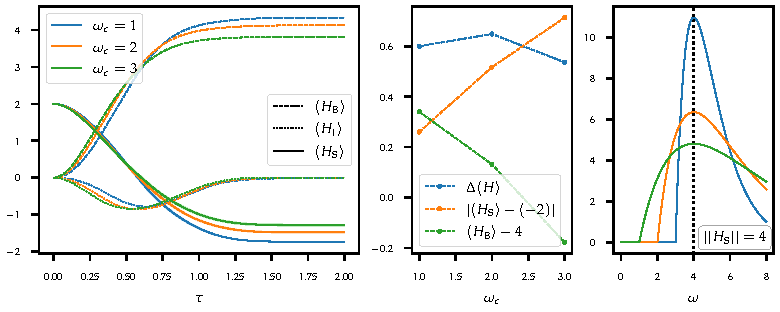
\includegraphics{figs/one_bath_syst/markov_analysis}
  \caption{\label{fig:markov_analysis} The same as
    \cref{fig:resonance_analysis} but for shifted spectral densities
    various bath memory times. The long-memory case performs best in
    this case, exhibiting the lowest final system energy.}
\end{figure}

Because the minimum in the interaction energy of the \(τ_{\bath}=1\)
case comes last, the residual interaction energy and thus interaction
strength is strongest when the interaction is turned off. Therefore
the largest quantity of energy is being introduced into the system in
this case when the interaction is disabled. In all cases the amount of
energy introduced is so large, that the bath energy slightly rises
during the decoupling process instead of falling as in
\cref{fig:resonance_analysis_steady}.


\begin{figure}[htp]
  \centering
  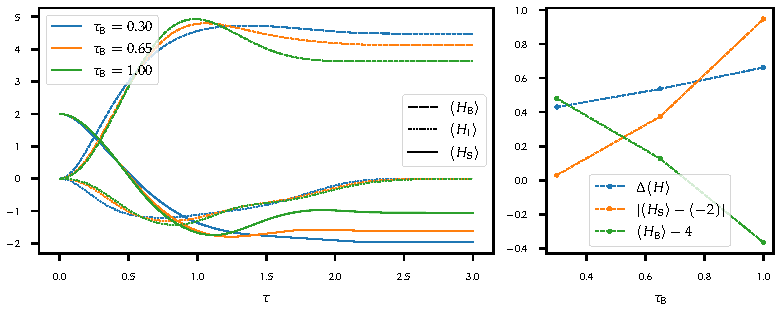
\includegraphics{figs/one_bath_syst/markov_analysis_longer}
  \caption{\label{fig:markov_analysis_longer} The same as
    \cref{fig:markov_analysis} but with slightly different timing. The
    result is exactly the reverse of
    \cref{fig:markov_analysis_longer}. Longer memories perform worse.}
\end{figure}
For slightly longer coupling times but with the same coupling
strengths, we find in the exact opposite picture as can be ascertained
from \Cref{fig:markov_analysis_longer}.  The increased bath memory
time allows for ``back flow'' of energy from the bath into the system
and so the performance of energy transfer is strongly dependent on the
precision of control. The oscillations of flow and thus bath energy
have already been noticed in \cref{sec:oneosccomp} and seem to be a
robust feature of stronger coupling and long bath
memories. \fixme{Append tables for model params.} The total energy
introduced is slightly less than for the short times as the
interaction energy is lower when the interaction is turned off.  The
final bath show an inverse behavior falling as the final system
energies rise. This is due to the energy transfer behavior, consistent
with the broadly similar total energy change in all three cases. This
behavior can also be observed \cref{fig:markov_analysis}.

For even longer times we find a picture similar to
\cref{fig:markov_analysis_steady}. The short memory case shows hardly
any backflow and performs best in terms of final system energy which
is extremely close to the target value of negative two. The other two
bath memories perform worse. We observe that simulation with the
longest bath memory stands out and having a very different final state
as is exemplified by the final system energy and the interaction
energy curve which exhibits a greater magnitude and persistent
oscillations.
\begin{figure}[htp]
  \centering
  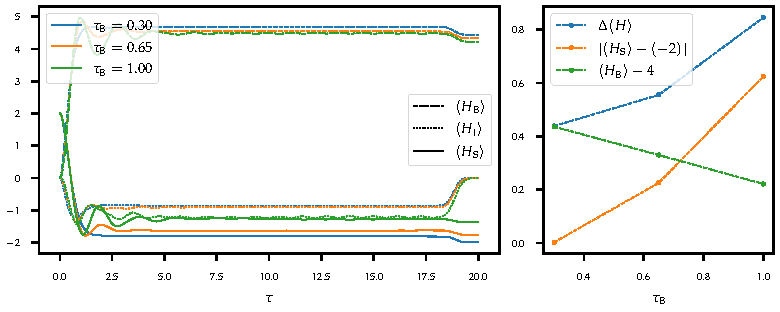
\includegraphics{figs/one_bath_syst/markov_analysis_steady}
  \caption{\label{fig:markov_analysis_steady} The same as
    \cref{fig:markov_analysis} but for long times. The results are
    broadly similar to \cref{fig:markov_analysis_longer} with the
    \(τ_{\bath}=1\) case standing out.}
\end{figure}

In the two simulations with shorter memory we find that about half of
the interaction energy is compensated by the total energy change. The
rest is accounted for by a lowering of system and bath energy alike,
an effect that is strongest in the short memory case especially for
the system energy. A slower, more adiabatic coupling modulation could
likely further reduce the amount of energy introduced.

As the steady state system energies\footnote{Before the interaction is
  switched off.} are greater than the ground state energies in all
simulations of \cref{fig:markov_analysis_steady} is a token of strong
coupling. The ground state is not the steady state, as it would be
with GKSL dynamics~\cite{Binder2018}.

We have often alluded to the fact that oscillations in the system
energy, the back-flow of energy into the system, are a token of
departure from the Markovian regime. An explicit demonstration of this
fact is given in \cref{fig:steady_relent}.

Spohn's theorem~\cite{Breuer2002Jun} states that the negative time
derivative of the relative entropy of system state and steady state
must be positive if the dynamics are generated by GKSL dynamics.
In mathematical terms Spohn's theorem can be formulated as
\begin{equation}
  \label{eq:spohn}
  -\dv{\qrelent{ρ_{\sys}(t)}{ρ_{\sys}(∞)}}{t} \geq 0,
\end{equation}
where \(\qrelent{ρ}{σ}=\tr[ρ \log_{2} ρ - ρ \log_{2} σ]\) is the
quantum relative entropy. The left hand side of \cref{eq:spohn} is
called entropy production.
\begin{figure}[htp]
  \centering
  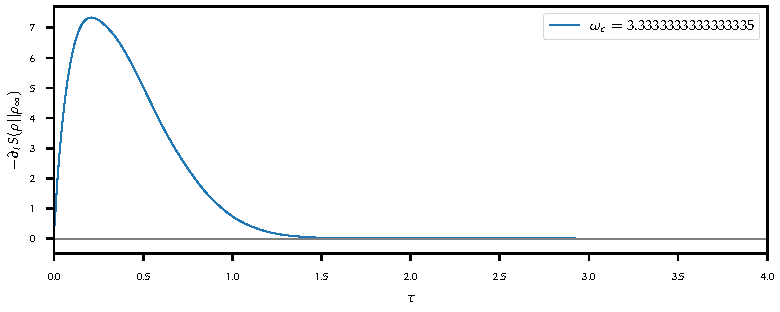
\includegraphics{figs/one_bath_syst/steady_relent}
  \caption{\label{fig:steady_relent} The negative time derivative of
    the relative entropy of system state and the approximate steady
    state (before the interaction is switched off) of the simulations shown in
    \cref{fig:markov_analysis_steady}. The short memory case does not
    violate Spohn's inequality, but the other two cases do. Note
    however, that the \(τ_{\bath}=1\) case has not yet reached a
    steady state and should therefore be treated with care.}
\end{figure}

\Cref{fig:steady_relent} demonstrates that the two simulations with
longer bathe memories are inconsistent with Markovian dynamics, as
their entropy production exhibits strong negativity. The
\(τ_{\bath}=1\) must be taken with care, as the steady state hasn't
been reached yet.

In summary we find that the energy dynamics of system, interaction and
bath depend strongly on the characteristics of the bath.  In the
regime studied, optimizing for fast energy loss of the system favors
longer bath memories, whereas the situation is reversed when longer
coupling times are allowed.

A resonance phenomenon has been observed which is already present in
the weak coupling case. However, here we additionally found a strong
dependence of the dynamics upon the shape of the whole spectral
density.

Note that the short time behaviour discussed here can usually not be
resolved by GKSL dynamics.

\paragraph{Initial Slip}
\begin{figure}[htp]
  \centering
  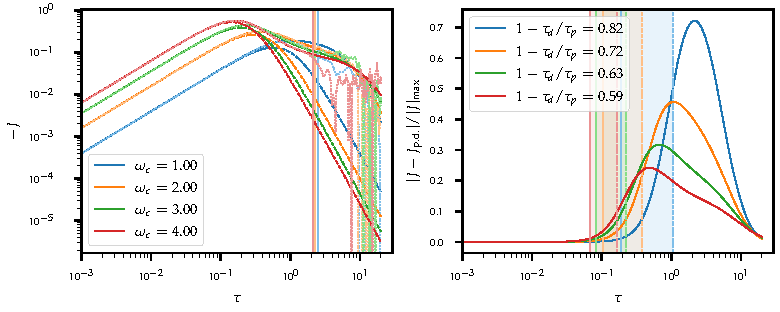
\includegraphics{figs/one_bath_syst/omega_initial_slip}
  \caption{\label{fig:omega_initial_slip} Left panel: The bath energy
    flow of the model \cref{eq:one_qubit_model} for various coupling
    strengths (solid lines) and the pure dephasing flow of
    \cref{sec:pure_deph} (dashed lines). The dotted lines show the
    flow calculated from one trajectory and the vertical lines mark
    the position of the peak of the absolute value of the interaction
    energy. Right panel: The difference of the actual flow \(J\) and
    the pure dephasing flow \(J_\mathrm{p.d.}\). The solid vertical
    lines mark the time \(τ_p\) where the normalized deviation from
    pure dephasing is \(10^{-2}\) and the dashed vertical lines show
    the position of the peak flow at time \(τ_p\). The divergence from
    pure dephasing dynamics occurs before the peak flow and the
    earlier the longer the bath memory. The single trajectory flow
    matches the converged flow for a longer period.}
\end{figure}

As the initial peak in the energy flow is also very prominent in the
simulations in this section we return to
\cref{fig:omega_systematics_system} and compare the dynamics of those
simulations to the pure dephasing case of \cref{sec:pure_deph}.

We see in \cref{fig:omega_initial_slip} that the pure dephasing
dynamics are accurate for very short time scales, but fail to predict
the exact location of the peaks in the bath energy flow. The deviation
from the pure dephasing flow occurs before the peak, where the time
difference between the absolute peak flow and the deviation increases
with increasing bath memory \(\propto 1/ω_c\), as does the magnitude
of the maximal relative deviation. This can be ascertained from the
legend of \cref{fig:omega_initial_slip} where the difference between
deviation and peak time normalized by peak time is given.

We can conclude that for longer bath memories along with weaker
couplings, the role of the system Hamiltonian dynamics in modulating
the flow becomes increasingly important as now the system dynamics
happen on the same time scale as the bath dynamics.

The flow calculated from a single trajectory matches the converged
longer than the pure dephasing flow. For large \(ω_{c}\) the single
trajectory matches until after the peak flow, whereas the deviation
occurs earlier for the \(ω_{c}=1\) case. The stochastic nature of the
single trajectory dynamics seems to become important only after a
finite amount of time, longer than period of pure dephasing
dynamics.

For short times the flow is mainly influenced by the buildup of the
auxiliary states rather than the fluctuations of the stochastic
process, leading to a similar behavior for most trajectories. See
\cref{fig:flow_buildup} an illustration of this phenomenon. This is
most useful, as this period of rapid dynamics must be resolved very
precisely to accurately integrate the flow into the bath energy
change.
\begin{figure}[htp]
  \centering
  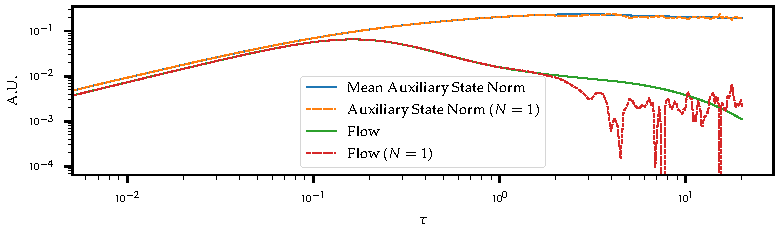
\includegraphics{figs/one_bath_syst/flow_buildup}
  \caption{\label{fig:flow_buildup} The total norm of the first
    auxiliary states and the flow for one trajectory and as a mean
    over all trajectories for the \(ω_{c}=4\) simulation. For short
    times the results for one trajectory match the ensemble means. The
    divergence between one trajectory and the ensemble occurs at
    roughly the same time for the flow and the auxiliary state
    norm. Moreover, flow and mean auxiliary state have the same
    functional form for very short times, apart from a scaling
    factor. The initial dynamics are therefore mainly concerned with
    populating the auxiliary states.}
\end{figure}

\subsection{Varying the Coupling Strength}
\label{sec:one_bathcoup_strength}
\begin{wrapfigure}[17]{O}{0.3\textwidth}
  \centering
  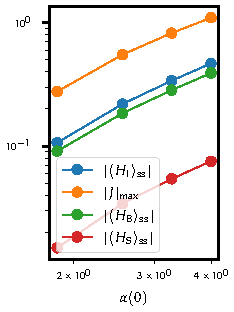
\includegraphics{figs/one_bath_syst/final_states_flows}
  \caption{\label{fig:delta_fs_flow} The absolute difference of the state energies and the
  maximal flows for the simulations in
  \cref{fig:delta_energy_overview} relative to their value at \(α(0)=1.12\).}
\end{wrapfigure}
After having studied the dependence of the bath energy flow for
various cutoff frequencies of the BCF in \cref{sec:one_bath_cutoff},
we now consider the case with fixed cutoff \(ω_c=2\) but varying
coupling strength. The results presented here are mainly a
demonstration of the feasibility of high-consistency simulations for a
range of coupling strengths. We will therefore keep the discussion of
the physical implications relatively short.

The chosen simulation parameters are the same as in
\cref{sec:one_bath_cutoff} and again consistent results have been
obtained as can be gathered from
\cref{fig:delta_interaction_consistency} throughout the whole range of
coupling strengths.
The interaction strength was chosen linearly spaced and the simulation
results are presented in \cref{fig:delta_energy_overview}.

As the shape of the BCF is not altered between the simulations, the
bath energy flows look very similar as do the interaction
energies. The main difference between the simulations is the magnitude
of the interaction energy. With increased coupling strength there is
an increased interaction energy and an increased flow which leads to
faster energy loss in the system and faster energy gain of the
bath. The stronger the coupling, the more pronounced is the
non-monotonicity in time of the interaction energy, which is reflected
in a non-monotonicity in the bath energy expectation value.

The bath energy reaches a maximum and falls slightly for the strongest
coupling simulations. If the interaction is strong enough,
``backflow'' can occur despite finite bath correlation times. In
\cref{fig:markov_analysis_steady} the bath memory is long,
additionally to a strong coupling so that multiple oscillations can be
seen.
\begin{figure}[htp]
  \centering
  \includegraphics{figs/one_bath_syst/δ_energy_overview}
  \caption{\label{fig:delta_energy_overview} Energy overview for the
    model \cref{eq:one_qubit_model} for various coupling
    strengths. The curves are converged out, and the error funnels are
    not visible.}
\end{figure}

Despite these differences for finite times, the approximate steady
state\footnote{excluding the \(α(0)=0.4\) cases} interaction energies,
maximal flows, system energies and bath energies are almost linearly
dependent on the coupling strength \(α(0)\) in this regime as is
demonstrated in the log-log plot \cref{fig:delta_fs_flow}.

We find that we can control the speed of the energy transfer between
bath and system with the coupling strength at the cost of greater
steady state interaction energy. Were we to turn off the interaction
very fast, we would have to expend this energy in the worst case. On
the other hand, more adiabatic protocol as the one used in
\cref{fig:markov_analysis_steady} would likely be a remedy to this
drawback.

The cooling performance for a coupling that is being turned off at the
end would depend on the concrete protocol as we've seen in
\cref{sec:one_bath_cutoff} and a more detailed study is left to future
work. The interplay between the interaction time-scale mediated by the
coupling strength, the bath memory time and the system dynamics allows
for intricate tuning.

Both the final system and bath energies are increasing with the
coupling strength, compensating for the interaction energy which is
the main mechanism that leads to residual system energy in the steady
state which is further and further away from the ground state, which
would be the steady state of weak coupling dynamics.


\fixme{iftime: re-run with same coupling strength, more cutoff freqs,
  less samples, see, longer times for coupling strengths, more coup}


\subsection{Moderating the Inital Slip with Modulated Coupling}
\label{sec:moder-init-slip}

\begin{wrapfigure}[17]{O}{0.4\textwidth}
  \centering
  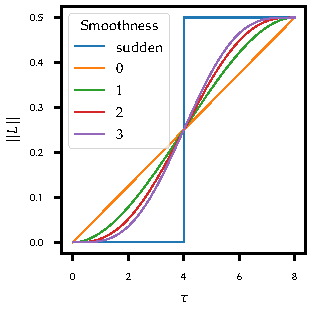
\includegraphics{figs/one_bath_mod/modulation_protocols_init.pdf}
  \caption{\label{fig:L_mod_init} The interaction is being switched on
    smoothly over a period of \(8\) time steps by the use of
    smoothstep functions (\cref{sec:smoothstep}) of different
    orders. A sudden protocol is being included for reference.}
\end{wrapfigure}
In \cref{sec:pure_deph} we derived the short term behavior of the
interaction dynamics by neglecting the system Hamiltonian. Up to now
we only have looked at the scenario in which the interaction is
present from the beginning. Now we will briefly demonstrate a case
where the interaction is switched on smoothly as in
\cref{fig:L_mod_init}.

The model is otherwise the same as \cref{eq:one_qubit_model}, where we
have chosen \(α(0)=1.6\) and \(ω_{c}=1\) for all the simulations. Some
\(N=10^{4}\) trajectories have been computed for each simulation.

The smoothness parameter \(s\) regulates to which order the derivative
of the modulation is continuous at \(t=0\) and \(t=8\). The modulation
of the coupling allows for a change in total energy. This leads to a
partial compensation for ``initial slip'' of the bath.

\begin{figure}[htp]
  \centering
  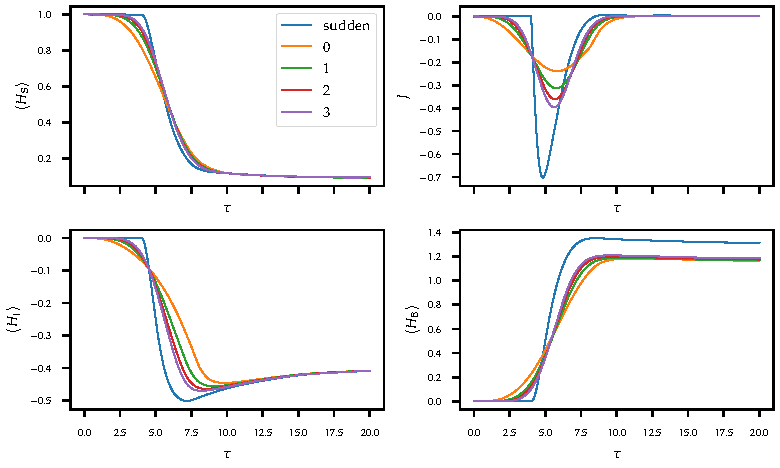
\includegraphics{figs/one_bath_mod/init_overview}
  \caption{\label{fig:init_energies}The relevant energy quantities for
    the different modulation protocols.}
\end{figure}
An overview over the bath system and interaction energy, as well as
the bath energy flow can be found in \cref{fig:init_energies}. System
and interaction energy all converge to the same values after some
time, but the bath energy is enhanced for the sudden case. This can
also been ascertained from the flow, which has a far greater magnitude
for this case.

The simulation with smoothness one exhibits a clear kink in the bath
energy flow and interaction energy curves at the time point \(τ=8\),
which reflects the lack of smoothness of the first derivative of the
modulation.

\cref{fig:init_total} shows that modulation protocols with a shallower
slope lead to a greater change in the total energy, compensating for
the negative interaction energy and leading to a shallower initial
slip flow.

The initial slip flow \cref{eq:pureflowexpectation} is valid for short
times, but the results diverge quite some time before peak flow.
\Cref{fig:init_slip_mod} demonstrates, that the qualitative properties
of the flow are still being capture quite well for short times.
\begin{figure}[htp]
  \centering
  \begin{subfigure}[t]{0.49\linewidth}
    \centering\captionsetup{width=.8\linewidth}
    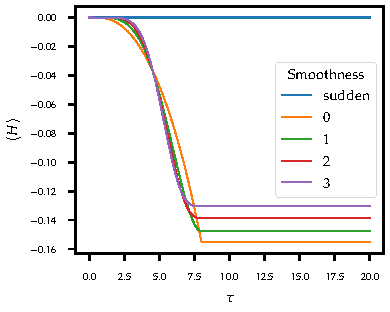
\includegraphics{figs/one_bath_mod/total_init}
    \caption{\label{fig:init_total}The total energy for different
      modulations. The slower the modulation, the more energy is
      released and the less energy is gained by the bath (see
      \cref{fig:init_energies}).}
  \end{subfigure}%
  \begin{subfigure}[t]{0.49\linewidth}
    \centering\captionsetup{width=.8\linewidth}
    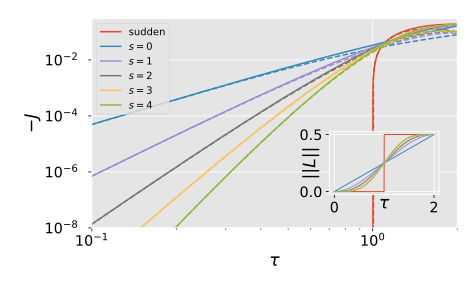
\includegraphics{figs/one_bath_mod/initial_slip_modcoup}
    \caption{\label{fig:init_slip_mod} The initial slip flow of
      \cref{eq:pureflowexpectation} and the exact flow. Initially, the
      flows coincidence, validating the earlier result. The flow peak
      heights and positions are being predicted incorrectly, but the
      initial slope and magnitude ordering are correct.}
  \end{subfigure}
  \caption{Total energy and flow for different interaction switching
    protocols.}
\end{figure}
